The goal of this chapter is to discuss the performance of Bacco, using a variery of parameters, methods and laboratory
tests. The results will also be compared to the ones obtained by applying the same procedures to devices using the
LoRaWAN protocol.

\section{Time On Air And Duty Cyle}
\Gls{ToA} is a crucial metric to take into consideration when measuring the performance of a network protocol. It is
defined as time that a device takes to transmit a packet on the channel. At the same conditions, a shorter \gls{ToA}
results in improved energy efficiency and smaller probability of interference with packets transmitted from other
devices.\\
\Gls{ToA} is correlated to the packet lenght in symbols (a longer packet will require a longer trasmission time).
Referencing the official LoRa documentation, see \cite{sx1262}, we can find that \gls{ToA} is
discussed in section 6.1.4; in particular the exact formula is shown here by Equation \ref{eqn: ToA}.
\begin{equation}
    \label{eqn: ToA}
    \mathit{ToA} = \frac{2^{\mathit{SF}}}{\mathit{BW}}*\mathit{N_{symbols}}
\end{equation}

where
\begin{itemize}[noitemsep,nolistsep]
    \item[\boldmath$\cdot$] $\mathit{SF}$ is the Spreading Factor (from 5 to 12);
    \item[\boldmath$\cdot$] $\mathit{BW}$ is the Bandwidth (in kHz);
    \item[\boldmath$\cdot$] $\mathit{N_{symbols}}$ is the number of symbols in the packet.
\end{itemize}
\\
$\mathit{N_{symbols}}$ can be calculated knowing the bytes of the packet ($\mathit{N_{bytes_{payload}}}$) using Equation \ref{eqn: n_symbols SF5_6} for $\mathit{SF} \in \left
\{5, 6 \right\} $ and Equation \ref{eqn: n_symbols SF7_12} for $\mathit{SF} \in \left
\[7, 12 \right\] $

\begin{equation}
    \label{eqn: n_symbols SF5_6}
    \resizebox{.9\hsize}{!}{
    \mathit{N_{symbols}} = \mathit{N_{symbols_{preamble}}} + 6.25 + 8 + \textit{ceil} \left( \frac{\textit{max} \left( 8 *
        \mathit{N_{bytes_{payload}}} + \mathit{N_{bits_{CRC}}} - 4 * \mathit{SF} + \mathit{N_{symbols_{header}}},
0 \right) }{\mathit{SF} * \mathit{CR}} \right)}
\end{equation}

\begin{equation}
    \label{eqn: n_symbols SF7_12}
    \resizebox{.9\hsize}{!}{
    \mathit{N_{symbols}} = \mathit{N_{symbols_{preamble}}} + 4.25 + 8 + \textit{ceil} \left( \frac{\textit{max} \left( 8 *
        \mathit{N_{bytes_{payload}}} + \mathit{N_{bits_{CRC}}} - 4 * \mathit{SF} + 8 + \mathit{N_{symbols_{header}}},
0 \right) }{\mathit{SF} * \mathit{CR}} \right)}
\end{equation}

where
\begin{itemize}[noitemsep,nolistsep]
    \item[\boldmath$\cdot$] $\mathit{N_{bits_{CRC}}}$ is number of bits used for \gls{CRC} and can assume a value of
        either 0 or 16;
    \item[\boldmath$\cdot$] $\mathit{N_{symbols_{header}}}$ is the number of symbols in the packet header.
        Since each symbol encodes $\mathit{SF}$ bits, $\mathit{N_{symbols_{header}}} = \frac{\mathit{N_{bits_{header}}}}
        {\mathit{SF}}$;
    \item[\boldmath$\cdot$] $\mathit{CR}$ is the coding rate and can assume a value of either $\frac{4}{5},\frac{4}{6},
        \frac{4}{7}$ or $\frac{4}{8}$.
\end{itemize}
\vspace{0.55cm}
The duty cycle is the fraction of time in which the channel is busy, it can be calculated using Equation \ref{eqn: duty cycle}.
\begin{equation}
    \label{eqn: duty cycle}
    d = \frac{\tau}{T}
\end{equation}
where
\begin{itemize}[noitemsep,nolistsep]
    \item[\boldmath$\cdot$] $d$ is the duty cycle;
    \item[\boldmath$\cdot$] $\tau$ is the \gls{ToA};
    \item[\boldmath$\cdot$] $T$ is the transmission period.
\end{itemize}
\\

\subsection{Regulations}
\label{subsec: regulations}
In order to maintain a fair distribution of the transmission activity, local, national and international governments
define limits on the usage of the radio channel. The limits vary by the frequency band in which the devices operate at.
The two parameters that are often used as an upper bound not to be crossed are \gls{ERP}\footnote{\gls{ERP} is the
measure of the power effectively radiated by an antenna system in a specific direction, accounting for both transmitter
output and antenna characteristic. It is commonly expressed in watts or decibel and it is used for determining the coverage area
and range of a radio.} and duty cycle.\\
Using the current Italian regulations at the time of writing as an example, we can observe that the spectrum is split into
frequency bands that can be either free, reserved or restricted; each of them has three parameters associated to it: the
maximum \gls{ERP}, the minimum channel bandwidth and the maximum duty cycle. The official document
that discusses this matter in detail can be found in \cite{gazzetta_potenza_868}. The bands that LoRa devices use in
Europe are $\[868.0,868.6\]$ MHz and $\[868.7,869.2\]$ MHz, they both feature a maximum \gls{ERP} of 25 mW or 14 dBm and
do not have any restriction on channel bandwidth, however the first band has a maximum duty cycle of 1\%, while for the
other the limit is set to 0.1\%.\\ An important fact to point out is that the limits apply to a physical person or
organization and not to on a device basis, so to calculate the effective duty cycle, we have to consider the
transmission activity generated by the whole network.

\subsection{Maximum Number Of Devices In A Network}
We can now calculate the maximum number of devices that can be operational at the same time. To achieve that, we can
derive Equation \ref{eqn: max devices rev} from Equation \ref{eqn: ToA} and then maximize the number of devices
($\mathit{N_{devices_{max}}}$), getting Equation \ref{eqn: max devices}.
\begin{equation}
    \label{eqn: max devices rev}
    \frac{\tau * \mathit{N_{devices}}}{T} \leq \mathit{d_{max}}
\end{equation}
\begin{equation}
    \label{eqn: max devices}
    N_{devices_{max}} = \textit{floor} \left( \frac{\mathit{d_{max}} * T}{\tau} \right)
\end{equation}
where
\begin{itemize}[noitemsep,nolistsep]
    \item[\boldmath$\cdot$] $T$ is the transmission period and can be set arbitrarily;
    \item[\boldmath$\cdot$] $\tau$ can be computed using Equation \ref{eqn: ToA};
    \item[\boldmath$\cdot$] $\mathit{d_{max}}$ is the maximum duty cycle, it has to be smaller or equal to 1 and can be
        set accordingly to the local regulations or the specific needs.
\end{itemize}
\\

\subsubsection{Example Of Calculation}
To demonstrate the use of the Equation \ref{eqn: max devices}, we will now consider a network with the following
properties:
\begin{itemize}
    \item each Sender node has a transmission period of $T = 1 \textit{ hour} = 3600\ s$;
    \item each Sender node transmits a packet with a payload that has a lenght in bytes equal to $\mathit{N_{bytes_{payload}}} = 16$;
    \item the network operates at a frequency of 868.0 Mhz on the Italian territory, and thus has to respect the limit
        of $\mathit{d_{max}} = 1\% = 0.01$.
\end{itemize}


\subsubsection{Bacco}
a downlink is sent every 10 packets;

\subsubsection{LoRaWAN}
a downlink is sent every packet (confirmation);


\section{Laboratory Tests}

\subsection{Single Packet Energy}

\begin{figure}[ht]
    \centering
    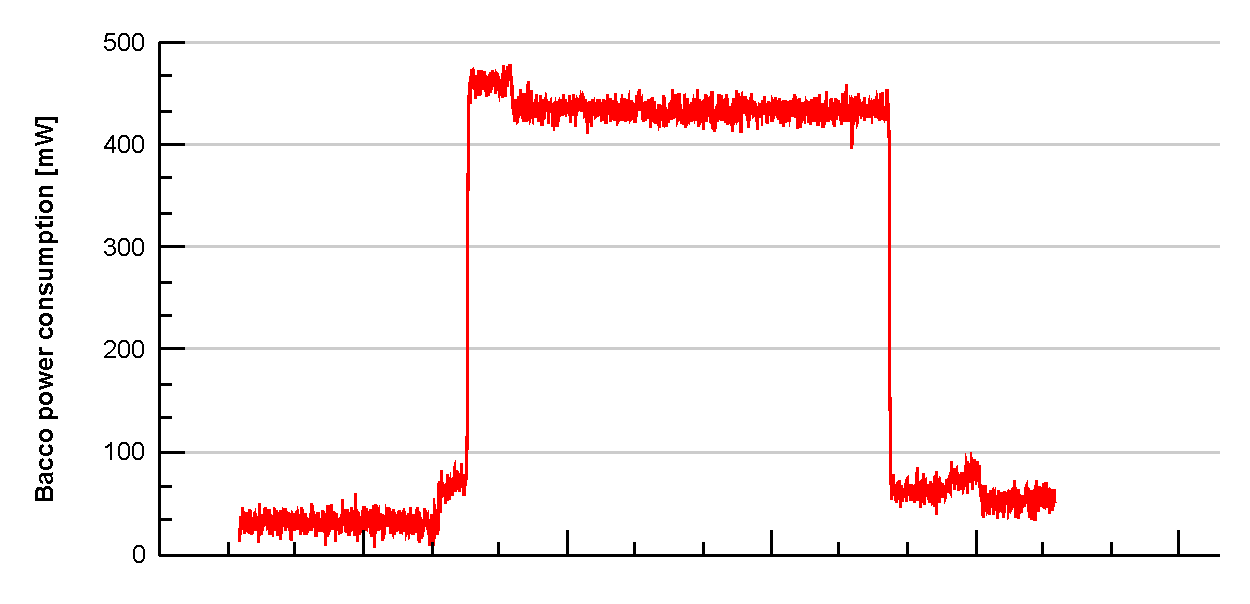
\includegraphics[width=1.0\textwidth]{images/bacco_SF7_14dbm_125khz_power.pdf}\\
    \vspace{-0.7cm}
    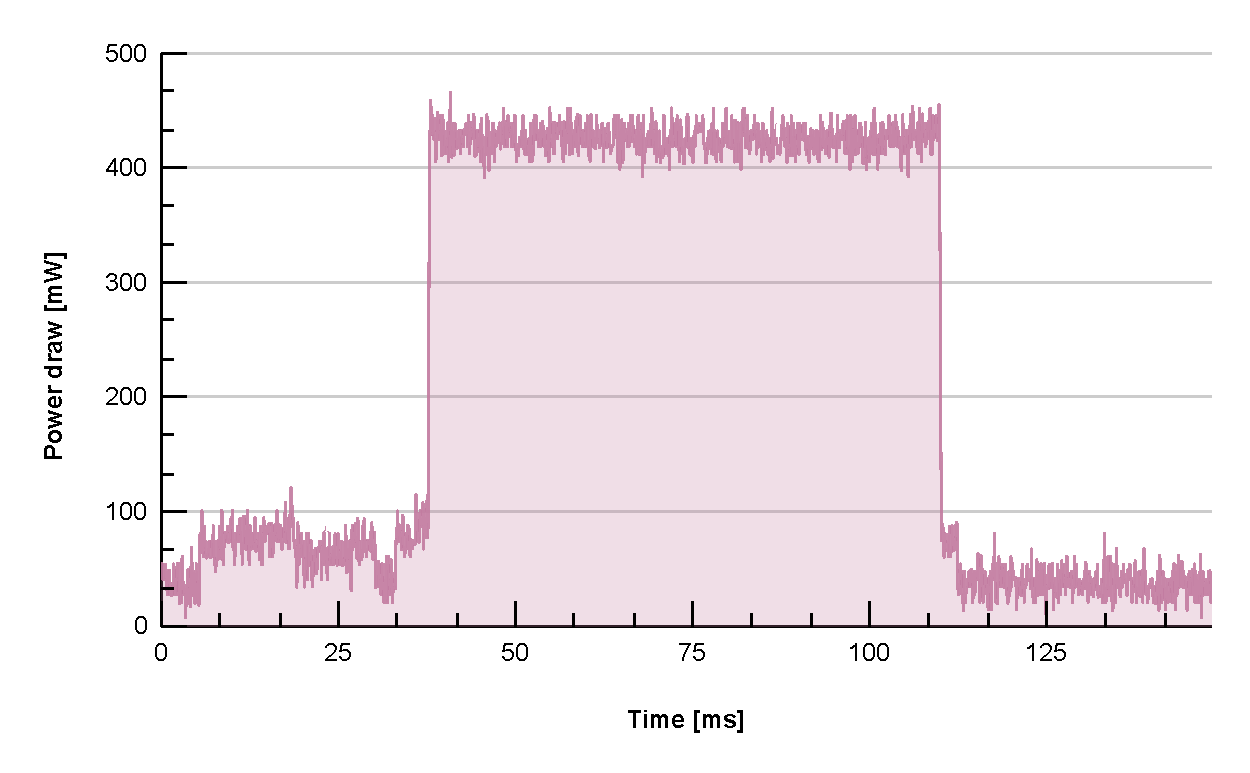
\includegraphics[width=1.0\textwidth]{images/lorawan_SF7_14dbm_125khz_power.pdf}
    \caption{Power draw of Bacco (in red) and LoRaWAN (in blue) during the transmission of a packet with a payload of 15
    bytes, using SF7, 14dBm, 125kHz bandwidth}
    \label{bacco SF7}
\end{figure}

Bacco:\\
delta time is 51.6ms and total energy is 21.3mJ
\\\\
LoRaWAN:\\
delta time is 71.8ms and total energy is 30.8mJ

\subsection{Packet Error Rate}
Crunch some fking data from FTP server

4 lost packets for every 1008 packets (0.4\% biatcz)
%TODO: similar test with fking LoRa fking WAN
